% !TeX root = mos-he.tex

%%%%%%%%%%%%%%%%%%%%%%%%%%%%%%%%%%%%%%%%%%%%%%%%%%%%%%%%%%%%%%%%

\begin{prob}{להכפיל את הדיוק}{}{(Doubling your accuracy)}

נתון שני מקלות באורכים
$L_1<L_2$
ומכשיר למדידת מרחק ששגיאת המדידה שלו ניתן על ידי התפלגות נורמלית עם ממוצע
$0$
ושונות
$\sigma^2$.
ניתן למדוד את אורכי המקלות על ידי מדידת כל מקל בנפרד. האם יש דרך מדוייקת יותר?
\end{prob}
\solution{}

\begin{figure}[bt]
\begin{center}
\begin{tikzpicture}
\draw (0,0) -- ++(6,0) -- ++(0,12pt) -- ++(-6,0) -- cycle;
\draw[<->] (0,24pt) --
  node[fill=white] {$\scriptstyle L_1+L_2$} ++(14,0);
\draw (6,0) -- ++(8,0) -- ++(0,12pt) -- ++(-8,0) -- cycle;
\begin{scope}[yshift=-48pt]
\draw (0,0) -- ++(8,0) -- ++(0,12pt) -- ++(-8,0) -- cycle;
\draw[yshift=12pt] (0,0) -- ++(0,12pt) -- ++(6,0) -- ++(0,-12pt);
\draw[<->] (6,20pt) --
  node[fill=white] {$\scriptstyle L_2-L_1$} ++(2,0);
\end{scope}
\end{tikzpicture}
\end{center}
\caption{מדידת האורכים של שני מקלות}\label{f.rods}
\end{figure}
הנח את המקלות קצה לקצה ומדד
$L_s=L_1+L_2$,
ואחר כך הנח את המקלות צד לצד ומדד
$L_d=L_2-L_1$ (איור%
~\ref{f.rods}).
חשב
$L_1,L_2$:
\begin{eqn}
\textstyle\frac{1}{2}(L_s-L_d)=\frac{1}{2}((L_1+L_2)-(L_2-L_1))&=&L_1\\
\textstyle\frac{1}{2}(L_s+L_d)=\frac{1}{2}((L_1+L_2)+(L_2-L_1))&=&L_2\,.
\end{eqn}
השגיאות במדידות הן
$e_s, e_d$
כך שהשגיאות התוצאות הן:
\begin{eqn}
\textstyle\frac{1}{2}((L_s+e_s)-(L_d+e_d))&=&L_1+\textstyle\frac{1}{2}(e_s-e_d)\\
\textstyle\frac{1}{2}((L_s+e_s)+(L_d+e_d))&=&L_2+\textstyle\frac{1}{2}(e_s+e_d)\,.
\end{eqn}
ממוצע של השגיאות במכשיר הוא
$0$
ולכן הממוצע של שתי המדידות גם כן $0$. השונות יורדת למחצית ערכה הקודמת:%
\footnote{%
המדידות בלתי-תלויות ולכן הקווריאנס הוא $0$.}
\begin{eqn}
\mathrm{Var}\left(\textstyle\frac{1}{2}\left(e_s-e_d\right)\right)&=&
  \textstyle\frac{1}{4}(\sigma^2+(-1)^2\sigma^2)=\frac{1}{2}\sigma^2\\
\mathrm{Var}\left(\textstyle\frac{1}{2}(e_s+e_d)\right)&=&
  \textstyle\frac{1}{4}( \sigma^2+\sigma^2)=\frac{1}{2}\sigma^2\,.
\end{eqn}


%%%%%%%%%%%%%%%%%%%%%%%%%%%%%%%%%%%%%%%%%%%%%%%%%%%%%%%%%%%%%%%%

\begin{prob}{משוואות ריבועיות אקראיות}{S}{(Random quadratic equations)}

תהי 
$x^2+2bx+c=0$
משוואה ריבועית המוגדרת מעל
$[-B,B]\times[-B,B]$
עבור
$B\geq 1$.

\que{1}
מה ההסתברות שהשורשים ממשיים?

\que{2} 
כאשר 
$B\rightarrow \infty$
מה ההסתברות שהשורשים ממשיים?
\end{prob}
\solution{}

\ans{1}
השורשים יהיו ממשיים אם הדיסקרימיננט 
$4b^2-4c\geq 0$
לא-שלילי. איור%
~\ref{f.real-roots}
מראה גרף של הפרבולה
$c=b^2$
כאשר השורשים המרוכבים נמצא בשטח האפור. למשל, עבור
$(b,c)=(1,2)$, 
ל-%
$x^2+2x+2$
שורשים מרוכבים (נקודה אדומה) ועבור
$(b,c)=(2,2)$
ל-%
$x^2+4x+2$
שורשים ממשיים (נקודה כחולה).

\begin{figure}[tb]
\begin{center}
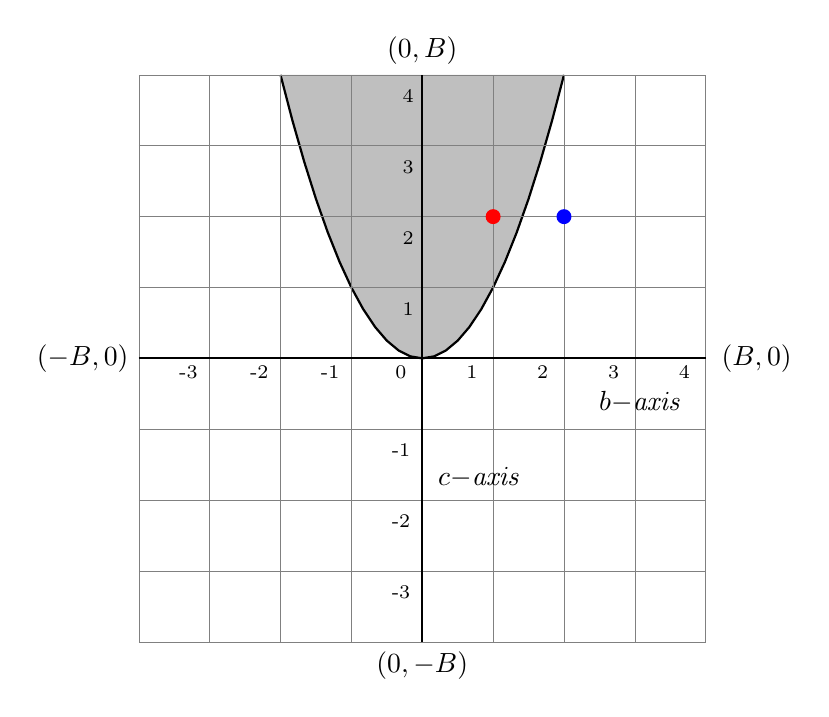
\begin{tikzpicture}[scale=.9]
\fill [white!50!gray, domain=-2:2]
      (-2, 4) -- plot ({\x}, {\x*\x}) -- (2, 4) -- cycle;
\draw [thick, domain=-2:2]
      (-2, 4) -- plot ({\x}, {\x*\x}) -- (2, 4);
\draw[help lines] (-4,-4) grid (4,4);
\draw[thick] (-4,0) -- (4,0);
\draw[thick] (0,-4) -- (0,4);
\foreach \x in {-3,...,4}
  \node at (\x-.3,-.2) {\scriptsize \x};
\foreach \y in {1,...,4}
  \node at (-.2,\y-.3) {\scriptsize \y};
\foreach \y in {-3,...,-1}
  \node at (-.3,\y-.3) {\scriptsize \y};
\draw[thick] (0,-4) node[below] {$(0,-B)$} -- 
  node[right,near start,xshift=2pt,yshift=8pt]
  {$c\mathit{-axis}$} (0,4) node[above] {$(0,B)$};
\draw[thick] (-4,0) node[left] {$(-B,0)$} --
  node[below,very near end,xshift=2pt,yshift=-8pt] 
  {$b\mathit{-axis}$} (4,0) node[right,xshift=2pt] {$(B,0)$};
\fill[red] (1,2) circle(3pt);
\fill[blue] (2,2) circle(3pt);
\end{tikzpicture}
\end{center}
\caption{%
עבור 
$(b,c)$
בשטח האפור השורשים של
$c=b^2$
מרוכבים}
\label{f.real-roots}
\end{figure}

נחשב את השטח האפור על ידי אינטגרציה:
\[
\int_{-\sqrt{B}}^{\sqrt{B}} (B-b^2)\,db=
\left. Bb-\disfrac{b^3}{3}\right|_{-\sqrt{B}}^{\sqrt{B}}=
\left(B^{3/2}-\frac{B^{3/2}}{3}\right)-
\left(-B^{3/2}+\frac{B^{3/2}}{3}\right)=
\disfrac{4}{3}B^{3/2}\,.
\]
השטח הכולל של
$[-B,B]\times[-B,B]$
הוא
$4B^2$
ולכן:
\begin{eqn}
P(\textrm{מרוכבים שורשים})&=&\disfrac{\frac{4}{3}B^{3/2}}{4B^2}=\disfrac{1}{3\sqrt{B}}\\
P(\textrm{ממשיים שורשים})&=&1-\disfrac{1}{3\sqrt{B}}\,.
\end{eqn}
\ans{2}
\[
\lim_{B\rightarrow\infty}
P(\textrm{ממשיים שורשים})=
\lim_{B\rightarrow\infty} \left(1-\disfrac{1}{3\sqrt{B}}\right)=
1\,.
\]

\textbf{סימולציה}
\selectlanguage{english}
\begin{verbatim}
For B =  4:
Probability of real roots = 0.8333
Proportion real roots     = 0.8271
For B = 16:
Probability of real roots = 0.9167
Proportion real roots     = 0.9205
For B = 64:
Probability of real roots = 0.9583
Proportion real roots     = 0.9582
\end{verbatim}
\selectlanguage{hebrew}

%%%%%%%%%%%%%%%%%%%%%%%%%%%%%%%%%%%%%%%%%%%%%%%%%%%%%%%%%%%%%%%%

\begin{prob}{הילוך מקרי דו-ממדי}{S}{(Two-dimensional random walk)}

חלקיק נמצא במרכז של מערכת צירים דו-ממדית. החלקיק צועד ימינה או שמאלה על ציר ה-%
$x$
עם הסתברות 
$1/2$
לכל כיוון 
\textbf{ובו-זמנית}
צועד למעלה או למטה על ציר ה-%
$y$
עם הסתברות 
$1/2$
לכל כיוון. איור%
~\ref{f.2d-random-walk}
מראה הילוך מקרי של 
$22$
צעדים שמתחיל ונגמר במרכז.

\que{1}
מה ההסתברות שהחלקיק חוזר למרכז ב-$2$ צעדים?

\que{2}
פתח נוסחה עבור ההתסתברות שהחלקיק חוזר למרכז (פעם אחת או יותר).

\que{3}
השתמש בקירוב של
\L{Stirling}
כדי לקבל הערכה של ההסתברות עבור $n$ גדול.

\begin{figure}[t]
\begin{center}
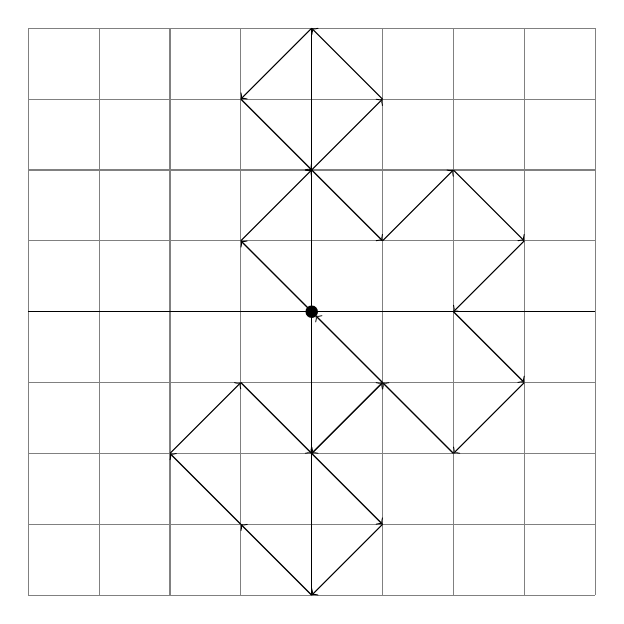
\begin{tikzpicture}[scale=.9]
\draw[color=gray] (-4,-4) grid (4,4);
\draw (-4,0) -- (4,0);
\draw (0,-4) -- (0,4);
\fill (0,0) circle[radius=2.5pt];
\draw[->] (0,0)  -- (-1,1);
\draw[->] (-1,1) -- (0,2);
\draw[->] (0,2)  -- (1,3);
\draw[->] (1,3)  -- (0,4);
\draw[->] (0,4)  -- (-1,3);
\draw[->] (-1,3) -- (0,2);
\draw[->] (0,2)  -- (1,1);
\draw[->] (1,1)  -- (2,2);
\draw[->] (2,2)  -- (3,1);
\draw[->] (3,1)  -- (2,0);
\draw[->] (2,0)  -- (3,-1);
\draw[->] (3,-1) -- (2,-2);
\draw[->] (2,-2) -- (1,-1);
\draw[->] (1,-1) -- (0,-2);
\draw[->] (0,-2) -- (1,-3);
\draw[->] (1,-3) -- (0,-4);
\draw[->] (0,-4) -- (-1,-3);
\draw[->] (-1,-3)-- (-2,-2);
\draw[->] (-2,-2)-- (-1,-1);
\draw[->] (-1,-1)-- (0,-2);
\draw[->] (0,-2) -- (1,-1);
\draw[->] (1,-1) -- (.055,-.055);
\end{tikzpicture}
\end{center}
\caption{הילוך מקרי דו-ממדי}\label{f.2d-random-walk}
\end{figure}
\end{prob}
\solution{}

\ans{1}
הנקודות באיור%
~\ref{f.two-moves}
מראות את המקומות האפשריים בהם החלקיק יכול להיות לאחר שני צעדים:
\begin{itemize}
\item
המסלול הירוק מראה איך להגיע ל-%
$(\pm 2, \pm 2)$
על ידי שני צעדים באותו כיוון. ההסתברות היא
$\left(\frac{1}{4}\right)^2= \frac{1}{16}$.
\item
המסלול האדום מראה איך להגיע ל-%
$(\pm 2,0)$
או ל-%
$(0,\pm 2$).
יש שני מסלולים אפשריים לכל נקודה ולכן ההסתברות היא
$2\cdot\left(\frac{1}{4}\right)^2= \frac{2}{16}$.
\item
המסלול הכחול מראה איך להגיע ל-%
$(\pm 1,\pm 1)$
ולחזור למרכז. ההסבתרות היא
$1/16$.
יש ארבעה מסלולים שחוזרים למרכז ולכן ההסתברות היא
$\frac{4}{16}$.
\end{itemize}
רק המסלולים הכחולים חוזרים למרכז ולכן:
\[
P(\textrm{צעדים בשני למרכז חזרה})=\frac{4}{16}\,.
\]

\begin{figure}[tb]
\begin{center}
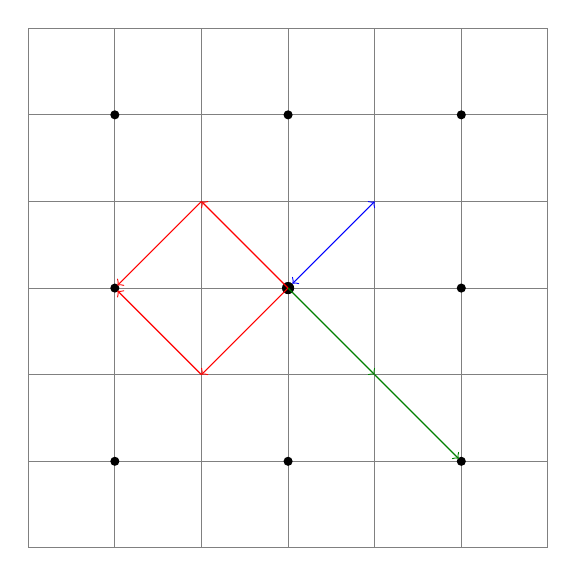
\begin{tikzpicture}[scale=1.1]
\draw[color=gray] (-3,-3) grid (3,3);
\fill (0,0) circle[radius=2pt];
\foreach \x/\y in {2/2, 2/-2, -2/2, -2/-2, 
                   0/2, 0/-2, 2/0, -2/0}
  \fill (\x,\y) circle[radius=1.5pt];
\draw[->,red] (0,0) -- (-1,-1);
\draw[->,red] (-1,-1) -- (-1.97,-.03);
\draw[<-,red] (-1.97,0.03) -- (-1,1);
\draw[<-,red] (-1,1) -- (0,0);
\draw[->,green!50!black] (0,0) -- (1,-1);
\draw[->,green!50!black] (1,-1) -- (1.97,-1.97);
\draw[<->,blue] (.05,.05) -- +(.95,.95);
%\draw[->,blue] (-0.1,0) -- +(1,1);
%\draw[->,blue] (1.1,1) -- +(-1,-1);
\end{tikzpicture}
\end{center}
\caption{שני צעדים בהילוך מקרי}\label{f.two-moves}
\end{figure}

\ans{3}
בחירת הכיוון בשני מצירים היא בלתי-תלויה כך שעבור
$2n$
צעדים:
\begin{equation}\label{eq.2d-1}
P_{2n}(\textrm{למרכז חזרה}) =
P_{2n}(x\!=\!0\textrm{ל- חזרה})\,P_{2n}(y\!=\!0\textrm{ל- חזרה})\,.
\end{equation}
החלקיק יחזור למרכז אם ורק אם בשני הצירים מספר הצעדים 
$+1$
שווה המספר צעדים
$-1$.
יש 
${2n \choose n}$
דרכים לסדר
$+1$
ו-%
$-1$
ולכן:
{
\addtolength{\arraycolsep}{-3pt}
\begin{eqnarray}
P_{2n}(x\!=\!0\textrm{ל- חזרה}) =P_{2n}(y\!=\!0\textrm{ל- חזרה})&=&
\dischoose{2n}{n}\left(\disfrac{1}{2}\right)^n\left(\disfrac{1}{2}\right)^{n}\\
P_{2n}(\textrm{למרכז חזרה}) &=&
\left[\dischoose{2n}{n}\left(\disfrac{1}{2}\right)^{2n}\right]^2\\
P(\textrm{למרכז חזרה}) =
\sum_{n=1}^{\infty}P_{2n}(\textrm{למרכז חזרה}) &=&
\sum_{n=1}^{\infty}\left[\dischoose{2n}{n}\left(\disfrac{1}{2}\right)^{2n}\right]^2\,.\label{eq.2d-2}
\end{eqnarray}
}
\ans{3}
לפי הקירוב של
\L{Stirling}
$n! \approx \sqrt{2\pi n}\left(n/e\right)^n$:
\begin{eqn}
P_{2n}(\textrm{למרכז חזרה}) &=&
\left[\dischoose{2n}{n}
\left(\disfrac{1}{2}\right)^{2n}\right]^2 \\
&=&
\left[\disfrac{(2n)!}{(n!)^2}
\left(\disfrac{1}{2}\right)^{2n}\right]^2 \\
&\approx&
\left(\disfrac{1}{2}\right)^{4n}
\disfrac{(\sqrt{2\pi \cdot 2n})^2
         \left(2n/e\right)^{4n}}
        {(\sqrt{2\pi n})^{4}
         \left(n/e\right)^{4n}} \\
&=&\left(\disfrac{1}{2}\right)^{4n}\disfrac{4\pi n}{4\pi^2 n^2}\cdot
\disfrac{\left(n/e\right)^{4n}\cdot 2^{4n}}{\left(n/e\right)^{4n}}\\
&=& \disfrac{1}{\pi n}\\
P(\textrm{למרכז חזרה}) &=& \disfrac{1}{\pi}\sum_{n=1}^{\infty}\disfrac{1}{n}\,,
\end{eqn}
שהיא
\textbf{סידרה הרמונית}
שמתבדרת, כלומר, עם הסתברות 
$1$
החלקיק חוזר למרכז!

\textbf{סימולציה}
הרצתי את הסימולציה מיליון פעמים במקום עשרת אלפים פעמים אבל התוצאה לא מראה שהחלקיק מגיע למרכז בוואדות.
\selectlanguage{english}
\begin{verbatim}
Proportion returned to origin      = 0.8700
\end{verbatim}
\selectlanguage{hebrew}

%%%%%%%%%%%%%%%%%%%%%%%%%%%%%%%%%%%%%%%%%%%%%%%%%%%%%%%%%%%%%%%%

\begin{prob}{הילוך מקרי תלת-ממדי}{D,S}{(Three-dimensional random walk)}

לקיק נמצא במרכז של מערכת צירים תלת-ממדית. החלקיק צועד ימינה או שמאלה על ציר ה-%
$x$
עם הסתברות 
$1/2$
לכל כיוון 
\textbf{ובו-זמנית}
צועד למעלה או למטה על ציר ה-%
$y$
עם הסתברות 
$1/2$
לכל כיוון.
\textbf{ובו-זמנית}
צועד פנימה או החוצה על ציר ה-%
$z$
עם הסתברות 
$1/2$
לכל כיוון.

\que{1}
מה
\textbf{התוחלת}
של מספר הפעמים שהחלקיק חוזר למרכז?

\textbf{רמז:}
חשב את ההסתברות ואחר כך תשתמש במשתנה מסמן
\L{(indicator variable)}.

\que{2}
מה ההסתברות שהחלקיק יחזור למרכז לפחות פעם אחת?

\textbf{רמז:}
תשתשמש בשיטה של בעיה~4.
\end{prob}
\solution{}

$P_{2n}$,
ההסתברות לחזור למרכז לאחר
$2n$
נתון על ידי הכללת משוואה%
~\ref{eq.2d-1}
לשלושה ממדים:
\[
P_{2n} =
P_{2n}(x=0\textrm{ל- חוזר})\,P_{2n}(y=0\textrm{ל- חוזר}\, P_{2n}(z=0\textrm{ל- חוזר})\,.
\]
$P_r$,
ההסתברות לחזור למרכז לפחות פעם אחת ניתנת על ידי הכללה לשלושה ממדים של משוואה%
~\ref{eq.2d-2}:
\[
P_r =\sum_{n=1}^{\infty}P_{2n} =
\sum_{n=1}^{\infty}\left[\dischoose{2n}{n}\left(\disfrac{1}{2}\right)^{2n}\right]^3\,.
\]
מהקירוב של
\L{Stirling}:\footnote{\L{Mosteller}
השתמש ב-%
$18$
איברים בחישוב שלו וקיבל
$0.315$.
התכנית שלי השתמש ב-%
$500$
איברים וקיבלתי
$0.3772$.}
\begin{eqn}
P_{2n} &=&
\left[\disfrac{(2n)!}{(n!)^2}
\left(\disfrac{1}{2}\right)^{2n}\right]^3 \\
&\approx&
\left(\disfrac{1}{2}\right)^{6n}
\disfrac{(\sqrt{2\pi \cdot 2n})^3
         \left(2n/e\right)^{6n}}
        {(\sqrt{2\pi n})^{6}
         \left(n/e\right)^{6n}} \\
&=&\disfrac{(4\pi n)^{3/2}}{(2\pi n)^3}=
 \disfrac{1}{(\pi n)^{3/2}}\\
P_r &=& \sum_{n=1}^{\infty}\disfrac{1}{(\pi n)^{3/2}}\approx 0.3772\,.
\end{eqn}
יהי 
$I_k$
משתנה מסמן עבור חזרה למרכז בצעד
$k$:
\begin{equation}
I_k=
\left\{
\begin{array}{ll}
1,\quad k\;\textrm{בצעד למרכז חוזר החלקיק אם}\\
0, \quad k\;\textrm{בצעד למרכז חוזר לא החלקיק אם}\,.
\end{array}
\right.
\end{equation}
אזי:
\[
E(\textrm{למרכז החזרות מספר})=\sum_{n=1}^{\infty}P_{2n}\, I_{2n} = P_r\approx 0.3772\,,
\]
ולכן התוחלת למספר החזרות למרכז שווה להסתברות.

\que{2}
תהי
$P_1$
ההסתברות שהחלקיק חוזר למרכז
\textbf{לפחות פעם אחת}.
מבעיה~4 אנו יודעים שהתוחלת של מספר בניסויים עד מראשון בו החלקיק 
\textbf{לא}
חוזר למרכז היא
$1/(1-P_1)$.
לכן, התוחלת של מספר הניסויים עד שהחליק כן חוזר למרכז היא אחד פחות, כי החלקיק יכול לחזור למרכז מספר רב של פעמים עד שהוא לא חוזר.%
\footnote{%
קשה לעקוב אחר הצגת הדברים של
\L{Mosteller}.
ברצוני להודית ל-%
\L{Aaron Montgomery}
שהבהיר לי את הפתרון
\L{\cite{montgomery}}.}

תהי
$E_r=E(\textrm{למרכז החזרות מספר})$. 
אזי:
\begin{eqn}
E_r &=& \disfrac{1}{1-P_1} - 1\\
P_1&=& \disfrac{E_r}{1+E_r}\,.
\end{eqn}
ב-%
\ansnc{1}
חישבנו ש-%
$E_r\approx 0.3772$
ולכן:
\[
P_1 \approx 1- \disfrac{1}{1+0.3772}
\approx 0.2739\,.
\]

\textbf{סימולציה}
\selectlanguage{english}
\begin{verbatim}
Expectation of reaching origin = 0.3772
Average times reached origin   = 0.3630
Probability of reaching origin = 0.2739
Proportion reached origin      = 0.2790
\end{verbatim}
\selectlanguage{hebrew}

%%%%%%%%%%%%%%%%%%%%%%%%%%%%%%%%%%%%%%%%%%%%%%%%%%%%%%%%%%%%%%%%

\begin{prob}{המחט של \L{Buffon}}{D,S}{(Buffon's needle)}

נתון משטח עם קווים מקביליים במרחק 
$1$
אחד מהשני. קח מחט באורך 
$a\leq 1$
וזרוק אותו על המשטח. מה ההסתברות שהמחט חוצה קו?%
\footnote{%
כדי להקל על החישובים אנו מניחים שהמרחק בין הקווים הוא 
$1$.
ניתן להתעלם מאפשרות שהמחט שוכב כולו לאורך אחד הקווים וכן את האפשרות שהוא נודע בשני קווים כי ההתסברות של אירועים אלה היא אפס.}

\textbf{רמז:}
יש שני משתנים אקראיים (איור%
~\ref{f.buffon1}): 
$x$,
המקום של מרכז המחט ביחס לקו הקרוב ביותר עם התפלגות אחידה בטווח 
$[0,1/2]$,
ו-%
$\theta$, 
הזווית שבין המחט לבין הקווים המקביליים עם התפלגות אחידה בטווח 
$[0,\pi/2]$.

\begin{figure}[tb]
\begin{center}
\begin{tikzpicture}[scale=.9]
\draw (0,0) -- (10,0);
\draw (0,4) -- (10,4);
\draw[<->] (1,0) -- node[fill=white] {$1$} (1,4);
\coordinate (center) at ($(4,-.5)+(60:1.5)$);
\node[above right,xshift=4pt] at (center) {$\theta$};
\node[above left] at (center) {$C$};
\draw[thick] (4,-.5) -- node[right,very near end] {$a$} +(60:4);
\draw[thick,dashed] ($(center)+(-2,0)$) -- +(6,0);
\draw[<->] (5.3,0) -- node[fill=white] {$x$}
  (center -| 5.3,0);
\end{tikzpicture}
\end{center}
\caption{המחט של\;Buffon}\label{f.buffon1}
\end{figure}
\end{prob}
\solution{1}

תהי 
$p(a)$
ההסתברות שמחט באורך 
$a$
חוצה קו והגדר משתנה מסמן:
\[
I_{\textrm{קו חוצה}}=
\left\{
\begin{array}{ll}
1,\quad \textrm{קו חוצה}\;a\;\textrm{באורך מחט}\\
0,\quad \textrm{קו לא חוצה}\;a\;\textrm{באורך מחט}\,.
\end{array}
\right.
\]
אזי:
\begin{equation}\label{eq.buffon-probability}
E(I_{\textrm{קו חוצה}})=1\cdot p(a) + 0\cdot (1-p(a))=p(a)\,,
\end{equation}
וניתן לחשב את ההסתברות על ידי חישוב התוחלת.

יהי 
$m$
אנח לקווים המקביליים שעובר דרך מרכז המחט ותהי 
$\theta$
הזווית בין המחט לבין אחד מהקווים המקביליים. הטל את המחט על 
$m$
כדי לקבל את הקטע הקו
$\overline{CD}$
(איור%
~\ref{f.buffon2}).
ההסתברות שהמחט חוצה קו היא:
\begin{equation}\label{eq.cross}
P(\textrm{קו חוצה}\;\theta\;\textrm{וזווית}\;a\;\textrm{באורך מחט})=\disfrac{(a/2)\sin \theta}{1/2}=a\sin\theta\,.
\end{equation}

\begin{figure}[bt]
\begin{center}
\begin{tikzpicture}[scale=1.5]
\draw (0,0) coordinate (O) -- (6,0);
\draw (0,2.5) -- (6,2.5);
\draw[<->] (.7,0) -- node[fill=white,near end] {$1$} +(0,2.5);
\draw[<->] (5,0) -- node[fill=white] {$1/2$} +(0,1.25);
\coordinate (end1) at (2,-.5);
\coordinate (end2) at ($(end1)+(60:3)$);
\coordinate (center) at ($(end1)+(60:1.5)$);
\draw[thick,dotted] (O |- center) -- +(6,0);
\draw[thick,dashed] (0,1.25) -- +(6,0);
\node[right,xshift=4pt,yshift=8pt]
  at (center) {$\theta$};
%\node[left,xshift=-4pt,yshift=-8pt]
%  at (center) {$\theta$};
\draw[thick,dashed] ($(center)+(0,-2)$) --
  node[right,very near end,xshift=-2pt,yshift=15pt]
  {$m$} +(0,4.2);
\node[right] at (end1 -| center) {$D$};
\node[left] at (end2-| center) {$C$};
\draw[thick] (end1) -- 
  node[left,near end] {$a/2$} (center) --
%  node[right] {$a/2$} 
  (end2);
\draw[thick] (end1) node[above right,xshift=4pt] {$\theta$} --
  (end1 -| center) --
  node[right,yshift=4pt] {$(a\sin\theta)/2$} (center);
\draw[thick] (end2) -- (end2 -| center) -- (center);
%\draw[thick] (end2) node[below left,xshift=-4pt] {$\theta$} --
%  (end2 -| center) -- 
%  node[left] {$(a\sin \theta)/2$} (center);
\end{tikzpicture}
\end{center}
\caption{משולש ישר-זווית לפתרון בעיית המחט של \L{Buffon}}
\label{f.buffon2}
\end{figure}

התוחלת של מספר הקווים שהמחט חוצה מתקבלת על ידי אינטגרציה מעל לזוויות האפשריות:
\begin{equation}\label{eq.buffon-integral}
E(\textrm{lines crossed}) =
  \disfrac{1}{(\pi/2)-0} \int_0^{\pi/2} a\sin \theta\,
  d\theta=\left.\disfrac{2}{\pi}\cdot a (-\cos \theta)
  \right|_0^{\pi/2}=\disfrac{2a}{\pi}\,.
\end{equation}

\solution{2}
הפתרון מבוסס על
\L{\cite[Chapter~26]{proofs}}.

\begin{figure}[tb]
\begin{center}
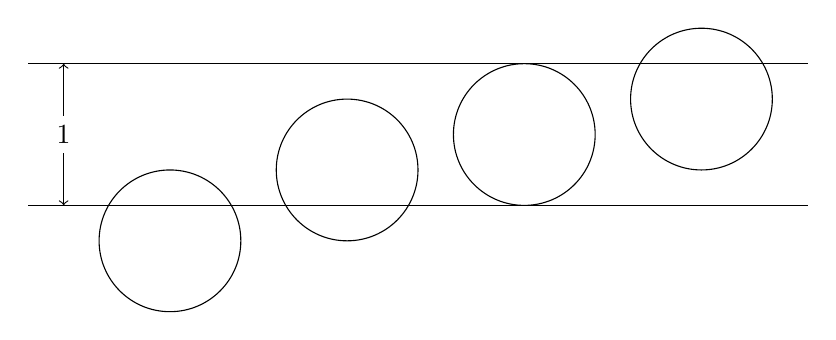
\begin{tikzpicture}[scale=.9]
\draw (0,0) -- (11,0);
\draw (0,2) -- (11,2);
\draw[<->] (.5,0) -- node[fill=white] {$1$} (.5,2);
\foreach \x/\y in {2/-.5, 4.5/.5, 7/1, 9.5/1.5}
  \draw (\x,\y) circle[radius=1];
\end{tikzpicture}
\end{center}
\caption{%
הפתרון של בעיית המחט של Buffon על מעגלים}
\label{f.buffon3}
\end{figure}

תהי 
$E(x)$
התוחלת שמ מספר הקווים המקביליים שקו באורך
$x$
חוצה. עיין עכשיו בקו שמסובבים למעגל
$C$
\textbf{בקוטר}
$1$
והיקף
$\pi$.
אם תזרוק את המעגל על המשטח, הוא יחצה קו 
\textbf{בדיוק}
פעמיים (איור%
~\ref{f.buffon3}),
ולכן:
\begin{equation}\label{eq.buffon-2}
E(C)=2\,.
\end{equation}
בנה מצולע משוכלל
$Q_n$
חסום על ידי 
$c$
(אדום), ובנה מצולע משוכלל 
$R_n$
שחוסם את
$c$
(כחול) (איור%
~\ref{f.buffon4}). 
כל קו ש-%
$Q_n$
חוצה (אדום) חייב לחצות את המעגל וכל קו שחוצה את המעגל (כחול) חייב לחצות את 
$R_n$.
לכן:
\begin{equation}\label{eq.buffon3}
E(Q_n)\leq E(C)\leq E(R_n)\,.
\end{equation}
יהי 
$a_Q, a_R$
סכומי באורכים של צלעות של
$Q_n,R_n$,
בהתאמה. לפי הליניאריות של התוחלת:
{
\addtolength{\arraycolsep}{-3pt}
\begin{eqnarray}\label{eq.buffon1a}
E(Q_n)&=&\sum_{i=1}^n E(a_Q\;\textrm{של צלעות})=a_QE(1)\\
\label{eq.buffon1b}E(R_n)&=&\sum_{i=1}^n E(a_R\;\textrm{של צלעות})=a_RE(1)\,. 
\end{eqnarray}
}
כאשר 
$n\rightarrow\infty$
שני המצולעים הם קירובים למעגל ולכן:
\begin{equation}\label{eq.buffon-pi}
\lim_{n\rightarrow\infty}a_Q = \lim_{n\rightarrow\infty} a_R=\pi\,,
\end{equation}
ההיקף של המעגל. ממשוואות%
~\ref{eq.buffon-2}--\ref{eq.buffon-pi}
מתקבל:
\[
\renewcommand*{\arraystretch}{1.5}
\begin{array}{l}
\lim_{n\rightarrow\infty}E(Q_n)=E(C) =\lim_{n\rightarrow\infty}E(R_n)\\
E(C)=aE(1) =\pi E(1) = 2\\
E(1)=\disfrac{2}{\pi}\\
E(a)=aE(1)=\disfrac{2a}{\pi}\,.
\end{array}
\]
\begin{figure}[bt]
\begin{center}
\begin{tikzpicture}
\draw[thick,green!80!black] (0,0) circle[radius=2];
\node[draw,red,thick] (in)
  [minimum size=4cm,regular polygon,regular polygon sides=6]
  at (0,0) {};
\node[draw,blue,rotate=30,thick] (out)
  [minimum size=4.62cm,regular polygon,regular polygon sides=6]
  at (0,0) {};
\node[above left,xshift=5pt] at (in.corner 5) {$Q_n$};
\node[below right,yshift=6pt] at (out.corner 5) {$R_n$};
\draw[thick,red] (-3,-.6) -- +(6,0);
\draw[thick,blue] (-3,1.9) -- +(6,0);
\end{tikzpicture}
\end{center}
\caption{מצולעים כקירובים למעדל}\label{f.buffon4}
\end{figure}

\textbf{סימולציה}

$\pi=2a/E$
ולכן ניתן לחשב קירוב לערכו על ידי הרצת סימולציה או זריקת מחטים על שולחן!
\selectlanguage{english}
\begin{verbatim}
For length = 0.2:
Expectation of crossings = 0.1273
Average crossings        = 0.1308
Empirical value for pi   = 3.0581

For length = 0.5:
Expectation of crossings = 0.3183
Average crossings        = 0.3227
Empirical value for pi   = 3.0989

For length = 1.0:
Expectation of crossings = 0.6366
Average crossings        = 0.6333
Empirical value for pi   = 3.1581
\end{verbatim}
\selectlanguage{hebrew}

%%%%%%%%%%%%%%%%%%%%%%%%%%%%%%%%%%%%%%%%%%%%%%%%%%%%%%%%%%%%%%%%

\begin{prob}{המחט של \L{Buffon} עם רשת אופקי ואנכי}{}{\\(Buffon's needle with horizontal and vertical rulings)}

פתור את בעיית המחט של 
\L{Buffon}
עבור משטח עם רשת אופקי ואנכי כאשר גודל המשבצות הוא 
$1\times 1$.
מחט יכול לחצות קו אנכי (ירוק), קו אופקי (כחול), שניהם (אדום) או אף אחד (כתום) (איור%
~\ref{f.buffon5}).

\begin{figure}[b]
\begin{center}
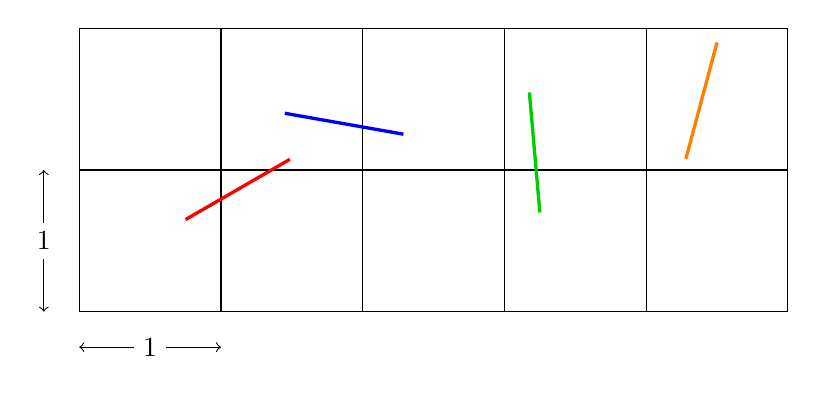
\begin{tikzpicture}[scale=.9]
\draw[step=2cm] (0,0) grid (10,4);
\draw[<->] (-.5,0) -- node[fill=white] {$1$} (-.5,2);
\draw[<->] (0,-.5) -- node[fill=white] {$1$} (2,-.5);
\foreach \x/\y/\a/\c in {
  1.5/1.3/30/red,
  2.9/2.8/-10/blue,
  6.5/1.4/95/green!80!black,
  9/3.8/-105/orange}
    \draw[color=\c,very thick] (\x,\y) -- +(\a:1.7);
\end{tikzpicture}
\end{center}
\caption{בעיית המחט של 
\L{Buffon}
עבור משטח עם רשת אופקי ואנכי}
\label{f.buffon5}
\end{figure}
\end{prob}
\textbf{רמז:}
האם מספר הקווים האופקים והאכנים שהמחט חוצה בלתי-תלויים?

\solution{}

מספר הקווים האופקים והאכנים שהמחט חוצה אכן בלתי-תלויים, ולפי הליניאריות של התוחלת:
\begin{eqn}
E(\textrm{חוצה}\; a\;\textrm{באורך שמחט קווים})&=&
E(\textrm{חוצה}\; a\;\textrm{באורך שמחט אנכים קווים}+\\
&&\quad\; \textrm{\textrm{חוצה}\; a\;\textrm{באורך שמחט אופקים קווים}})\\
&&E(\textrm{חוצה}\; a\;\textrm{באורך שמחט אנכים קווים})+\\
&&E(\textrm{\textrm{חוצה}\; a\;\textrm{באורך שמחט אופקים קווים}})\\
&=&\disfrac{2a}{\pi}+\disfrac{2a}{\pi}=\disfrac{4a}{\pi}\,.
\end{eqn}


%%%%%%%%%%%%%%%%%%%%%%%%%%%%%%%%%%%%%%%%%%%%%%%%%%%%%%%%%%%%%%%%

\begin{prob}{מחטים ארוכים}{D,S}{(Long needles)}

יהי 
$a>1$
אורכו של המחט בבעייתו של
\L{Buffon}.

\que{1}
מה התוחלת של
\textbf{מספר הקווים}
שמחט חוצה?

\que{2} 
מה ההסתברות שהמחט חוצה
\textbf{לפחות}
קו אחד?

\textbf{רמז:}
עבור איזו זוויות 
$\theta$
ההסתברות של חציית קו היא
$1$?

\end{prob}
\solution{}

\ans{1}
שבור את המחט לחלקים באורים
$\{a_1,a_2,\ldots, a_n\}$, $a_i< 1$,
כך ש-%
$\sum_{i=1}^n a_i=a$.
לפי הליניאריות של התוחלת והפתרון של בעיה~53:
\[
E(a)= \sum_{i=1}^n E(a_i)= \disfrac{2a}{\pi}\,.
\]

\ans{2}
הפתרון מבוסס על
\L{\cite{wiki-buffon}}
ו-%
\L{\cite[Chapter~26]{proofs}}.

לפי משוואה%
~\ref{eq.cross}
ההסתברות שהמחט יחצה קו היא
$a\sin\theta$ 
\textbf{אם}
$a\sin\theta \leq 1$,
כלומר, אם
$0\leq\theta\leq\sin^{-1}(1/a)$.
אבל, אם
$a\sin\theta > 1$
ההסתברות היא
$1$
(איור%
~\ref{f.buffon6}).
נכליל את משוואה%
~\ref{eq.buffon-integral}
עבור
$a>0$
שרירותי. האינטגרל מוחשב בשני חלקים, אחד עבור
$\theta<\sin^{-1}(1/a))$
ואחר עבור
$\theta>\sin^{-1}(1/a))$:
\begin{eqn}
E(a) &=& \disfrac{2}{\pi}
   \left(\int_{0}^{\sin^{-1}(1/a)} 
   a\sin \theta\:d\theta + 
   \int_{\sin^{-1}(1/a)}^{\pi/2} 1\: d\theta\right)\\
&=& \disfrac{2}{\pi}\left(\left.
    a(-\cos \theta)\right|_0^{\sin^{-1}(1/a)} + 
    \left(\disfrac{\pi}{2} - 
    \sin^{-1}(1/a)\right)\right)\\
&=& 1+\disfrac{2}{\pi}
  \left(a
  \left(1-\sqrt{1-\disfrac{1}{a^2}}\right)-
  \sin^{-1}(1/a)\right)\,.
\end{eqn}

\begin{figure}[tb]
\begin{center}
\begin{tikzpicture}[scale=1]
\draw (0,0) -- (10,0);
\draw (0,3.5) -- (10,3.5);
\draw[<->] (.5,0) -- node[fill=white,near end] {$1$} +(0,3.5);
\draw[<->] (5.5,0) -- node[fill=white] {$1/2$} +(0,1.75);
\begin{scope}[xshift=0cm,yshift=1.4cm,scale=1]
\coordinate (end1) at (2,-1);
\coordinate (end2) at ($(end1)+(60:3)$);
\coordinate (center) at ($(end1)+(60:1.5)$);
\node[above right,xshift=2pt,yshift=-2pt]
  at (end1) {$\theta$};
\draw (end1) --  node[left,near end] {$a/2$} (center) -- (end2);
\draw (end2) -- (end2 -| center);
\draw (end1) -- (end1 -| center);
\draw[very thick] (end1 -| center) -- 
  node[right,fill=white,yshift=2pt] {$(a/2)\sin \theta$}
  (center) -- (end2 -| center);
\draw[thick,dotted] (O |- center) -- +(10,0);
\end{scope}
\begin{scope}[xshift=3cm,yshift=.8cm,scale=1.6]
\coordinate (end1) at (2,-1);
\coordinate (end2) at ($(end1)+(60:3)$);
\coordinate (center) at ($(end1)+(60:1.5)$);
\node[above right,xshift=2pt,yshift=-2pt]
  at (end1) {$\theta$};
\draw (end1) --  node[left,near end] {$a/2$} (center) -- (end2);
\draw (end2) -- (end2 -| center);
\draw (end1) -- (end1 -| center);
\draw[very thick] (end1 -| center) -- 
  node[right,fill=white,yshift=6pt] {$(a/2)\sin \theta$}
  (center) -- (end2 -| center);
\end{scope}
\end{tikzpicture}
\end{center}
\caption{מחטים ארוכים}\label{f.buffon6}
\end{figure}

\textbf{סימולציה}
\selectlanguage{english}
\begin{verbatim}
For length = 1.5:
Expectation of crossings = 0.7786
Average crossings        = 0.7780
For length = 2.0:
Expectation of crossings = 0.8372
Average crossings        = 0.8383
For length = 3.0:
Expectation of crossings = 0.8929
Average crossings        = 0.8897
\end{verbatim}
\selectlanguage{hebrew}

%%%%%%%%%%%%%%%%%%%%%%%%%%%%%%%%%%%%%%%%%%%%%%%%%%%%%%%%%%%%%%%%

\begin{prob}{הכד של \L{Molina}}{}{(Molina's urns)}

שני כדים
$U_1,U_2$
מכילים 
$m$
כדורים כל אחד. ב-%
$U_1$
נמצאים 
$w_1$
כדורים לבנים ו-%
$b_1$
כדורים שחורים, וב-%
$U_2$
נמצאים
$w_2$
כדורים לבנים ו-%
$b_2$
כדורים שחורים. מכל כד שלוף
$n$
כדורים
\textbf{עם החזרה}.

\que{1}
עבור ערכים שונים של
$n>1$
מצא
$w_1,b_1,w_2,b_2$
כך ש:
\[
P(\textrm{לבנים}\;U_1\textrm{מ- שנשלפו כדורים כל})=
P(\textrm{שחורים או לבנים}\;U_2\textrm{מ- שנשלפו כדורים כל})\,.
\]
\end{prob}
\solution{}

\ans{1}
עבור 
$n=2$
המשוואה שיש לפתור היא:
\begin{eqn}
\left(\disfrac{w_1}{m}\right)^2&=&\left(\disfrac{w_2}{m}\right)^2+\left(\disfrac{b_2}{m}\right)^2\\
w_1^2&=&w_2^2+b_2^2\,.
\end{eqn}
פתרון אחד הוא
$w_1=10,b_1=4,w_2=6,b_2=8$.

\ans{2}
לפי המשפט האחרון של
\L{Fermat},
שהוכח ב-%
$1995$
על ידי
\L{Andrew Wiles},
אין פתרונות ל-%
$w_1^n=w_2^n+b_2^n$ 
עבור
$n\geq 3$.

%%%%%%%%%%%%%%%%%%%%%%%%%%%%%%%%%%%%%%%%%%%%%%%%%%%%%%%%%%%%%%%%

